\documentclass[serif, aspectratio=169]{beamer}
%\documentclass[serif]{beamer}  % for 4:3 ratio

\RequirePackage{minted2}
\usepackage[T1]{fontenc} 
\usepackage[utf8]{inputenc}
\usepackage{fourier} % see "http://faq.ktug.org/wiki/uploads/MathFonts.pdf" for other options
\usepackage{hyperref}
\usepackage{latexsym,amsmath,xcolor,multicol,booktabs,calligra}
\usepackage{graphicx,pstricks,listings,stackengine}
\usepackage{lipsum}
\usepackage{../HKUSTstyle}

%imports customs%
\usepackage{caption}    % for subfigures
\usepackage{subcaption} % for subfigures
\usepackage{ragged2e}
\usepackage{booktabs,makecell}
\usepackage{colortbl}
\usepackage{multirow}
\usepackage{cite}
\usepackage{tcolorbox}
\usepackage[sort,authoryear]{natbib}

\author{Julien Bezançon}

\title{Python Programmation}
\subtitle{CM 4~: Data Manipulation}

\institute{julien.bezancon@univ-lorraine.fr / \url{https://julienbez.github.io}}

\date{}

% defs
\def\cmd#1{\texttt{\color{red}\footnotesize $\backslash$#1}}
\def\env#1{\texttt{\color{blue}\footnotesize #1}}

% set colors
\definecolor{hkustyellow}{RGB}{167, 131, 55}
\definecolor{hkustblue}{RGB}{0, 56, 116}
\definecolor{hkustred}{RGB}{209, 51, 59}

\lstset{
    basicstyle=\ttfamily\small,
    keywordstyle=\bfseries\color{deepblue},
    emphstyle=\ttfamily\color{deepred},    % Custom highlighting style
    stringstyle=\color{deepgreen},
    numbers=left,
    numberstyle=\small\color{halfgray},
    rulesepcolor=\color{red!20!green!20!blue!20},
    frame=shadowbox,
}

\begin{document} %  --- --- --- --- --- --- --- --- --- --- --- --- 

\begin{frame}[noframenumbering,plain]
    \titlepage
    \vspace*{-0.6cm}
    \begin{figure}[htpb]
        \begin{center}
            \hspace{0.3cm}
            
\includegraphics[width=0.7\columnwidth]{../../../IMAGES/loria_idmc.png}
        \end{center}
    \end{figure}
\end{frame}

% \begin{frame}    
%     \tableofcontents[sectionstyle=show,
%     subsectionstyle=show/shaded/hide,
%     subsubsectionstyle=show/shaded/hide]
% \end{frame}

\section{Before we start...}

\begin{exoframe}
    \begin{center}
        \Large
        What did you learn during last lecture ? \\
        Any questions ?
    \end{center}
\end{exoframe}

\begin{frame}{Last Lecture Doggy bag}
    \begin{minipage}{0.45\columnwidth}

    \end{minipage}
    \hfill
    \begin{minipage}{0.45\columnwidth}
        \begin{figure}
            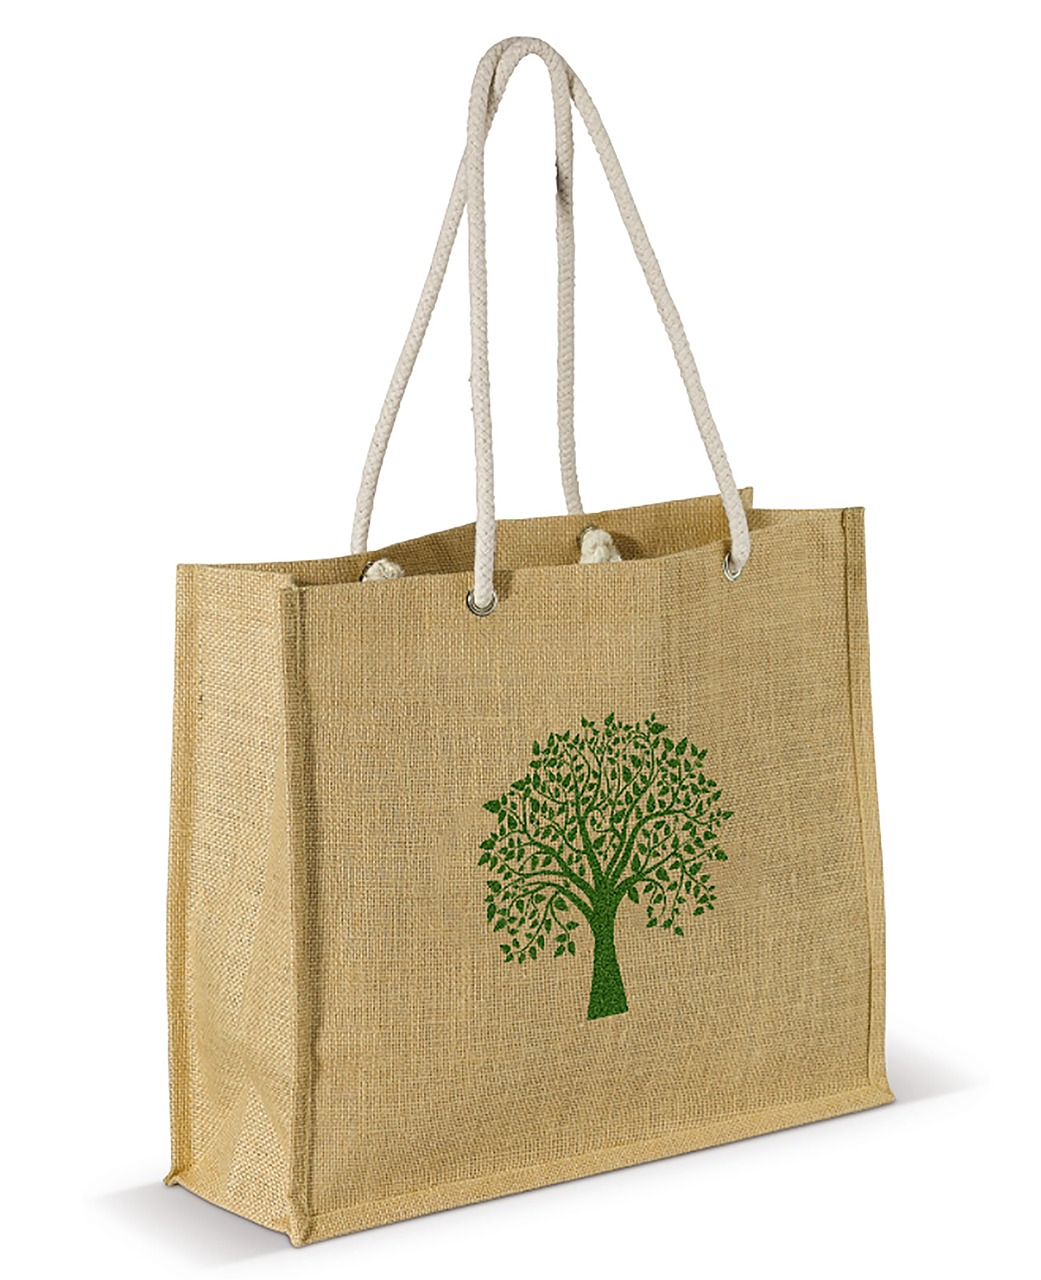
\includegraphics[width=0.9\columnwidth]{../../../FIGURES/divers/doggybag.jpg}
        \end{figure}
    \end{minipage}
\end{frame}

\section{Data Formats}

% \begin{frame}{Data Types}
%     \begin{block}{You already know about data types}
%         \begin{itemize}
%             \item Integer (int)
%             \item String (str)
%             \item Float (float)
%             \item Boolean (bool)
%             \item List (list)
%             \item etc
%         \end{itemize}
%     \end{block}
%     \vspace{10pt}
%     \begin{center}
%         \Large
%         You can think of them as categories to store similar values.
%     \end{center}
% \end{frame}

\begin{frame}
    %human-readable vs machine readable format
    %compromises = can be read by humans but has a strict structure to facilitate navigation with a machine
    % example : markup languages => set of rules to combine with desired content to create a format both readable by a human and easily manipulable by a machine
    %add image of a codebarre + image of a markup language (HTML ?) + image of human readable format 
\end{frame}

\begin{frame}
    %frame about encoding informations in a file
    % when writing a data, it is saved in in bytes, you ENCODE it to bytes 
    % a byte is a contiguous sequence of bits => 00000110 (6)
    % several files encoding = several ways of encoding data to bytes, you must be careful when encoding files => most common = UTF-8
    % format => describes a set of valid sequences of symbols. When applied to the bytes of a file, it open it correctly
\end{frame}

\begin{frame}
    % extensions => txt, json, cvs, tsv, parquet, ...
    % the extension indicate the format to use when reading a file => how to read the bytes in a file 
    % show most common formats and say that we are going to work with them in python
\end{frame}

\begin{frame}
    % text format => very simple,
\end{frame}

\end{document}